\documentclass[a4paper,10pt]{article}

%Packages
\usepackage{txfonts}
\usepackage{titlesec}
\usepackage[utf8]{inputenc}
\usepackage[T1]{fontenc}
\usepackage{geometry}
\usepackage{graphicx}
\usepackage{lipsum}
\usepackage{multicol}
\usepackage{fancyhdr}
\usepackage{hyperref}
\usepackage{float}
\usepackage{setspace}
\usepackage{caption}
\usepackage{booktabs}

% PAGE LAYOUT
\geometry{a4paper, top=18mm, bottom=18mm, textwidth=185mm}
\setlength{\columnsep}{6mm}
\setlength{\parindent}{0pt}

\titleformat{\section}
{\normalfont\bfseries}
	{\thesection.}{0.5em}{}
\titleformat{\subsection}
	{\normalfont\itshape}
	{\thesubsection.}{0.5em}{}

\pagestyle{fancy}
\renewcommand{\footrulewidth}{0pt}
\fancyhf{}
\rhead{
\includegraphics[scale=0.4]{Images/hepia_simple.png}}
\rfoot{\textit{\today}}
\cfoot{\thepage}

\captionsetup{
  font=footnotesize,
  labelsep=colon
}

\begin{document}

\begin{multicols*}{2}
[
\begin{center}
\vspace*{0mm}
{\large
AI in Healthcare data -- Module 1\\
\vspace{3mm}
Data Preparation, Summarization, Visualization, Reduction and \\
Diagnostic Performance Analysis of a Prostate Cancer Cohort
}\\
\vspace{8mm}
Guilhem Rozier Vilardell\footnote{\textit{\href{mailto:guilhem.roziervi@hes-so.ch}{guilhem.roziervi@hes-so.ch}}}
\\
\vspace{3mm}
\footnotesize{
\textit{AI in Healthcare Summer Camp -- Module 1: Data Preparation, Summarization, Visualization and Reduction}
}\\
\vspace{9mm}
\end{center}
\rule{\linewidth}{0.4pt}
\onehalfspacing
\textbf{Abstract}\\
Three raw datasets describing a prostate cancer (PC) cohort -- demographic/clinical records, biochemical laboratory values, and coded comorbidity diagnoses -- were cleaned, type-corrected, and merged into a single analysis-ready dataset (1{,}159 patients, 25 variables). Missing biochemical values were imputed and the resulting panel was summarized descriptively and by correlation structure. Prostate-specific antigen (PSA) was then evaluated as a diagnostic marker of metastasis at two fixed cutoffs and across its full range via ROC analysis (AUC = 0.670), and the ten biochemical markers were reduced to three principal components (PC1--PC3, 69.3\% cumulative variance) using PCA. Results show PSA has moderate, cutoff-dependent discriminative power, and that the biomarker panel is compressible with limited information loss.\\
\noindent\textit{Keywords:} prostate cancer, PSA, missing data, ROC curve, PCA, biomarker panel\\
\rule{\linewidth}{0.4pt}
]
\singlespacing

\tableofcontents

\setlength{\parskip}{1pt}
\columnbreak
% INTRODUCTION
\section{Introduction}

Prostate cancer (PC) is a disease that happens to a large proportion of the population. the goal of this research is to explore the use of AI to help in the diagnosis of prostate cancer. 
Until now, diagnosis and follow-up rely on heterogeneous data: clinical records, laboratory records, and medical history. the first step in any data analysis is to prepare the data for modeling.\\
Before any of this data can support diagnostic or prognostic modelling, it must be inspectedand understood. to help us we will manipulate the data by type-corrected, checked for missingness, merged into a coherent structure, and -- where the number of correlated biomarkers is large -- reduced to a smaller, more tractable set of components.\\
This report covers this data cleaning phase, feature selection and classification. data preparation, summarization, visualization and diagnostic performance and data reduction of the AI in Healthcare summer camp.

The two questions that interest us are: (i) how should missing and heterogeneous data from three separate sources be prepared into a single reliable cohort table, and (ii) how well does prostate-specific antigen (PSA), alone, discriminate patients who go on to develop metastasis, and can the wider biomarker panel be compressed without losing much information.

% DATA
\section{Data}

Three source files, identified by patient \texttt{ID}, were provided.

\textbf{DATASET1 -- clinical data}: civil status, family history of cancer, metastasis status (outcome), and three date fields (first PC diagnosis, metastasis diagnosis, birth date).

\textbf{DATASET2 -- laboratory data}: ten numeric laboratory markers (monocyte, urea, lymphocyte, thrombocyte, erythrocyte, albumin, creatinine, globulin, PSA, coagulation factor).

\textbf{DATASET3 -- medical history}: one row per diagnosed condition per patient, using condition codes (diabetes, hearing loss, hypercholesterolaemia, hypertension, osteoporosis, urinary retention).

% METHODS
\section{Data Preparation and Methods}
The first step is to understant what does this data represent? do the values make sense? are there any missing values? are the data types correct?\\
The second step is to prepare the data for analysis. this includes type correction, missing data handling, recoding and reshaping, merging, imputation, correlation structure analysis, PSA diagnostic performance analysis, and principal component analysis (PCA).

\subsection{Type correction}
In DATASET1, civil status, cancerfamily and metastasis were re-typed from integer to categorical, and the three date columns were parsed as datetimes. DATASET2's dtypes were already appropriate and left unchanged.
DATASET3

\subsection{Missing data}
DATASET1's only missingness was in the metastasis-diagnosis date (738/1{,}159 = 63.7\% missing). It's expected since patients without metastasis have no such date. A filtered check confirmed zero patients with \texttt{metastasis=1} and a missing date, i.e. no unexplained (semantic) missingness. DATASET2 showed scattered missingness across biochemical markers (0.3--14.1\% per column, worst in lymphocyte), visualized with a missingness bar chart and matrix (Fig.~\ref{fig:missbar} and\ref{fig:missmat}).

\begin{figure}[H]
\centering
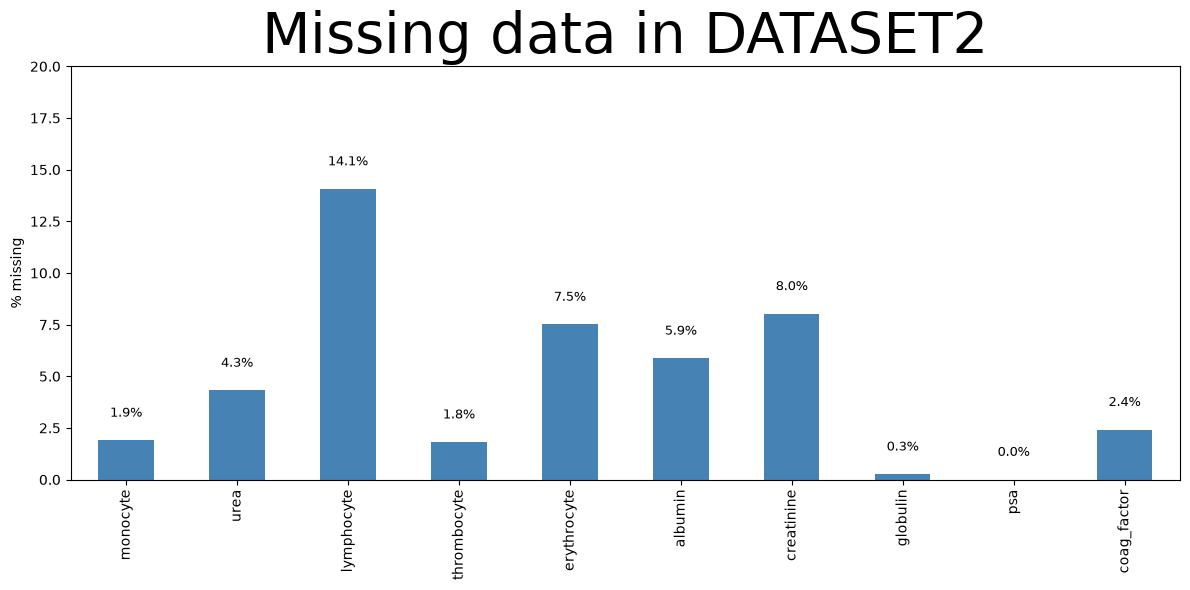
\includegraphics[width=\linewidth]{Images/missing_bar.png}
\caption{Missing-value percentage per biochemical variable, DATASET2.}
\label{fig:missbar}
\end{figure}



\subsection{Recoding and reshaping}
DATASET3's six codes were mapped to disease labels and pivoted from long format (one row per diagnosis) to wide format (one row per patient, one binary column per disease), using \texttt{pivot\_table} with \texttt{max} aggregation.

\subsection{Merging}
DATASET1, DATASET2, and the wide disease table were left-joined on \texttt{ID} (base = DATASET1, so every original patient is retained even if a comorbidity table entry is absent). Post-merge, disease columns with \texttt{NaN} (patient absent from DATASET3, i.e. no diagnosis on record) were set to 0. Result: \texttt{DATASET123}, 1{,}159 rows $\times$ 25 columns.

\subsection{Imputation}
Most of the histograms (Fig.~\ref{fig:hist}) appear skewed and present outliers, with the exceptions being thrombocyte and erythrocyte, whose distributions appear quite balanced and symmetrical. Therefore, median imputation was chosen as most suitable for the majority of the biochemical markers.

\begin{figure}[H]
\centering
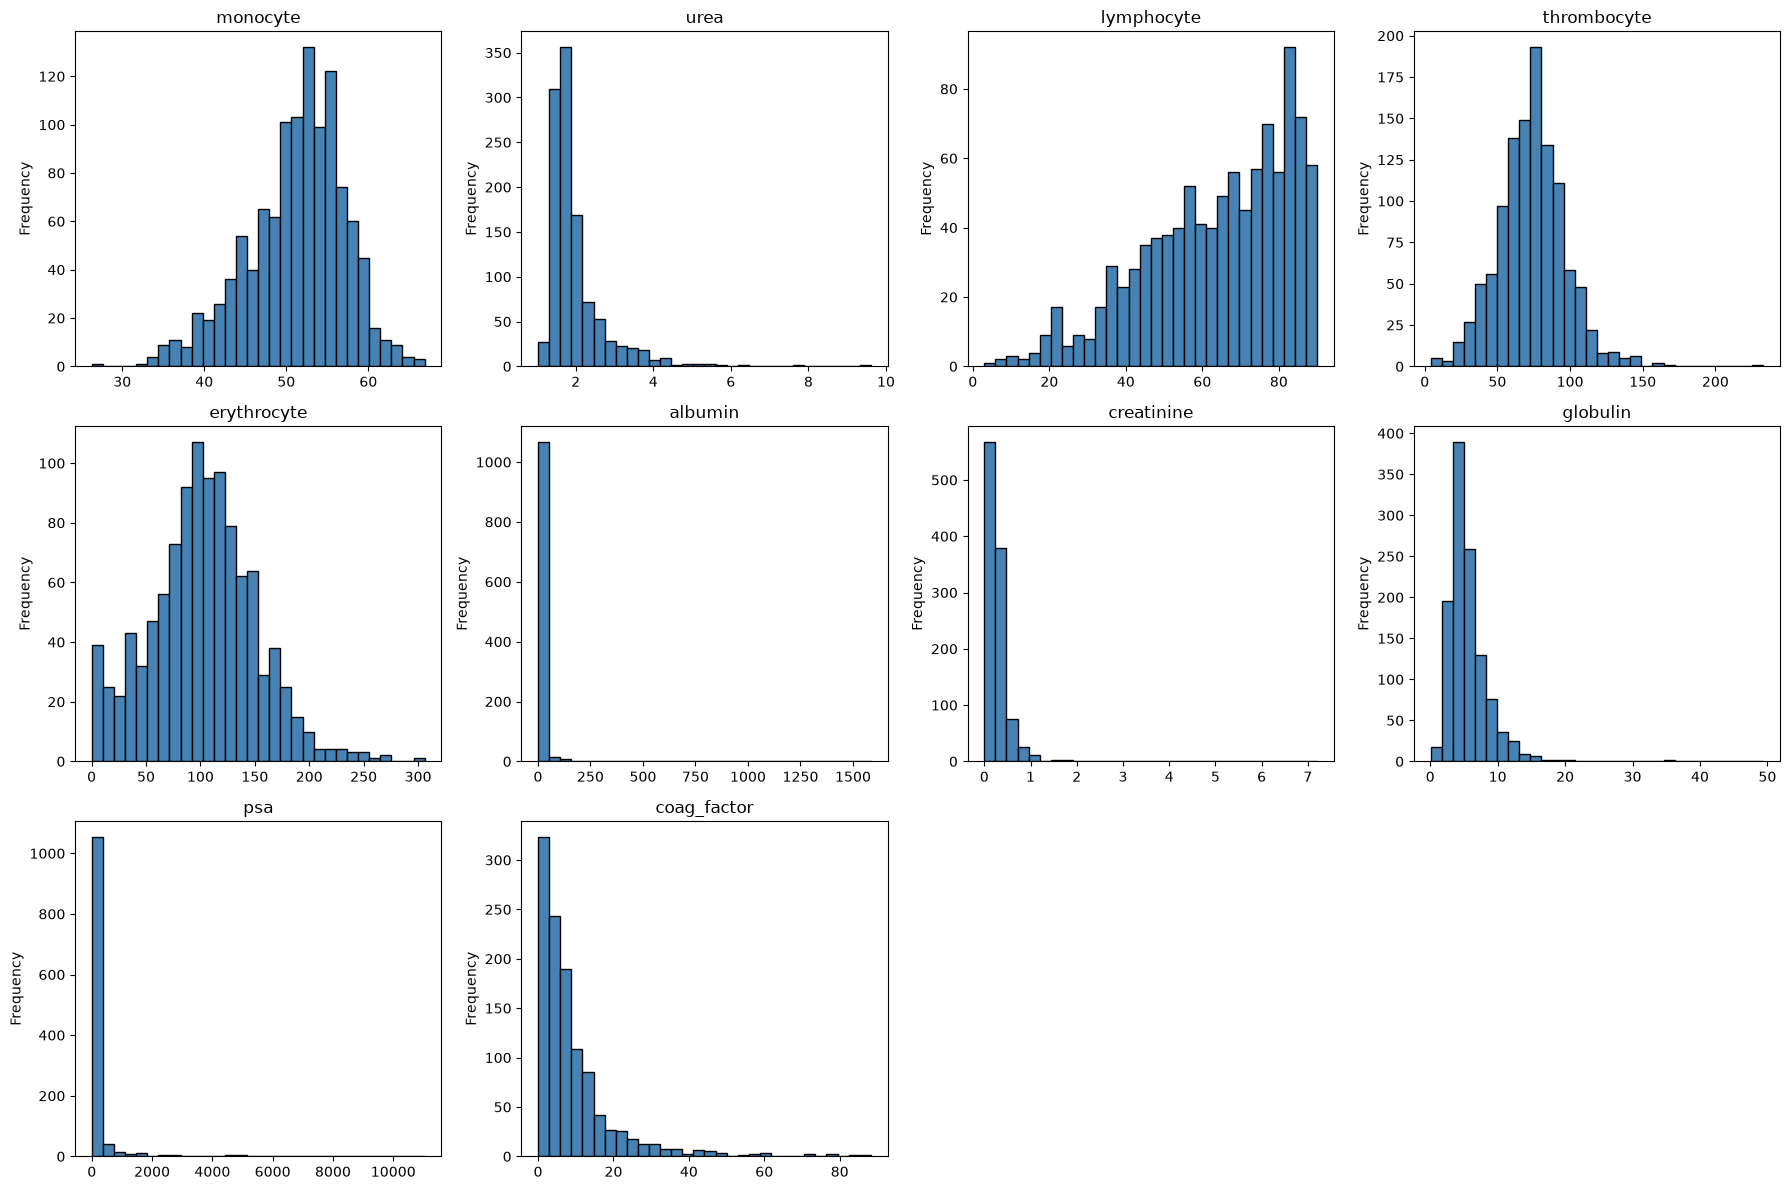
\includegraphics[width=\linewidth]{Images/biomarker_hist.png}
\caption{Distribution of the ten biochemical markers (DATASET2), used to select an imputation method.}
\label{fig:hist}
\end{figure}

\subsection{Correlation structure}
Pairwise Pearson correlations between the ten biomarkers were computed and visualized as a heatmap (Fig.~\ref{fig:corr}) to check for redundancy before PCA.

\begin{figure}[H]
\centering
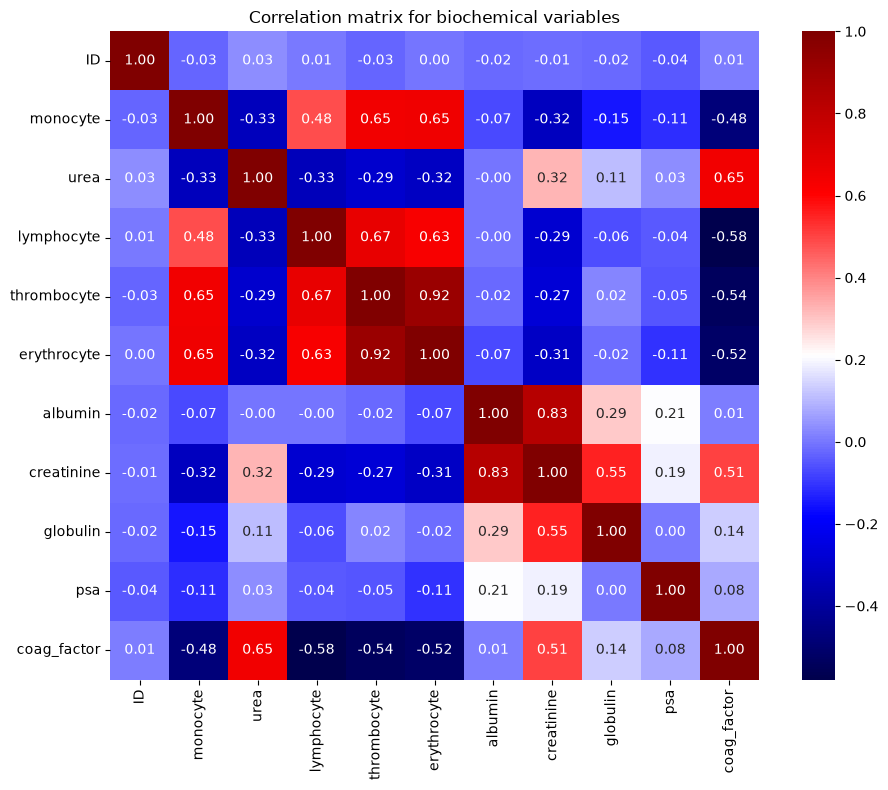
\includegraphics[width=\linewidth]{Images/corr_heatmap.png}
\caption{Correlation matrix of the ten biochemical markers.}
\label{fig:corr}
\end{figure}
The correlation matrix illustrates the degree to which the biochemical variables in DATASET2 co‑vary, revealing a generally modest pattern of linear associations. Most pairwise correlations cluster around zero, indicating that the majority of variables behave largely independently of one another. A few moderate correlations are visible, suggesting biologically plausible relationships — for example, parameters linked to hematologic or renal function show mild positive or negative associations, though none approach the strength typically required to imply redundancy or multicollinearity. Importantly, the absence of strong correlations (i.e., values approaching ±1) suggests that the dataset does not contain highly collinear predictors, and thus each variable contributes distinct informational value. Overall, the correlation structure supports the use of these variables in multivariable analyses without substantial risk of instability due to interdependence.

\subsection{ATTENTION: PSA diagnostic performance}
Metastasis was used as the ground-truth label. Two fixed PSA cutoffs (20 and 100~ng/mL) were tested by building binary test-result columns and computing sensitivity, specificity and accuracy against the confusion matrix. A full receiver operating characteristic (ROC) analysis was then run using PSA as a continuous score, and the optimal cutoff was located two ways: (i) the Youden index ($\mathrm{TPR}-\mathrm{FPR}$, maximized), and (ii) class-size-weighted maximum accuracy.

\subsection{ATTENTION: Principal Component Analysis}
The ten biomarkers were standardized (zero mean, unit variance, since PCA is scale-sensitive) and decomposed with PCA. Components were retained using the eigenvalue$>1$ (Kaiser) criterion.

% RESULTS
\section{Results}

\subsection{Patient characteristics}
Table~\ref{tab:characteristics} summarizes the cohort derived from DATASET1.

\begin{table}[H]
\centering
\caption{Patient characteristics (N = 1{,}159).}
\label{tab:characteristics}
\begin{tabular}{lr}
\toprule
Variable & Value \\
\midrule
Age at PC diagnosis (yr) & 74.3 $\pm$ 8.7 \\
Age at metastasis (yr)$^{*}$ & 78.9 $\pm$ 8.5 \\
Metastasis: yes & 421 (36.3\%) \\
Metastasis: no & 738 (63.7\%) \\
Family history of cancer: yes & 623 (53.8\%) \\
Family history of cancer: no & 536 (46.2\%) \\
Civil status: married/cohabiting & 808 (69.7\%) \\
Civil status: single/divorced/widowed & 351 (30.3\%) \\
\bottomrule
\end{tabular}\\
\footnotesize{$^{*}$computed on the 421 patients with metastasis.}
\end{table}

Roughly one in three patients in the cohort developed metastasis. The age at metastasis diagnosis is on average $\sim$4.6 years older than age at initial PC diagnosis, consistent with metastasis typically occurring after initial diagnosis rather than at presentation.

\subsection{Missing data and correlation}
Missingness in DATASET2 is modest overall (0.3--14.1\%) and, per Fig.~\ref{fig:missmat}, scattered rather than block-patterned -- supporting the use of simple imputation over multiple imputation or case deletion. The correlation heatmap (Fig.~\ref{fig:corr}) shows mostly weak pairwise correlations, with only a few moderate associations plausibly linked to shared hematologic/renal physiology; no pair approaches $|r|\approx1$, so variable dependencies is not a major concern for downstream modelling.

\subsection{Merged dataset}
\texttt{DATASET123} (1{,}159 $\times$ 25) combines clinical, laboratory and medical history information per patient. The left-join on the DATASET1 base guarantees no patient is lost even when a source table lacks an entry for them; filling missing disease flags with 0 encodes "no diagnosis on record" rather than "unknown," which is the appropriate default for a comorbidity registry built from positive diagnostic codes only.

\subsection{PSA at fixed cutoffs}
Table~\ref{tab:psa} reports performance at the two pre-specified PSA thresholds.

\begin{table}[H]
\centering
\caption{PSA diagnostic performance at two fixed cutoffs.}
\label{tab:psa}
\begin{tabular}{lcc}
\toprule
 & PSA $>$20 ng/mL & PSA $>$100 ng/mL \\
\midrule
Sensitivity & 0.596 & 0.323 \\
Specificity & 0.672 & 0.867 \\
Accuracy & 0.645 & 0.670 \\
\bottomrule
\end{tabular}
\end{table}

The low cutoff maximizes sensitivity (catches more true metastatic cases, more false alarms); the high cutoff maximizes specificity (few false alarms, misses roughly two-thirds of metastatic cases). Accuracy is similar for both ($\sim$0.65--0.67) because it is pulled toward the majority (non-metastatic) class, illustrating why accuracy alone is a poor criterion for choosing a cutoff in an imbalanced cohort.

\subsection{ROC analysis and optimal cutoff}

\begin{figure}[H]
\centering
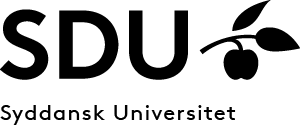
\includegraphics[width=\linewidth]{Images/roc_curve.png}
\caption{ROC curve for PSA as a continuous predictor of metastasis. AUC = 0.670.}
\label{fig:roc}
\end{figure}

AUC = 0.670 indicates moderate discrimination -- better than chance (0.5) but well below what is expected of a strong single-marker test ($\gtrsim$0.9). The two cutoff-selection criteria disagree substantially: the Youden index selects 23~ng/mL (sensitivity 0.582, specificity 0.694), close to the pre-specified 20~ng/mL cutoff, while maximum accuracy selects 134~ng/mL (accuracy 0.679), close to the pre-specified 100~ng/mL cutoff. This mirrors the fixed-cutoff result: Youden weighs sensitivity and specificity equally, while class-weighted accuracy favours the majority (non-metastatic) class and therefore specificity.

\subsection{Principal Component Analysis}
By the eigenvalue$>1$ criterion, 3 components were retained (eigenvalues 3.90, 1.95, 1.10; the 4th drops to 0.93), jointly explaining 69.3\% of total variance in the ten-marker panel (Fig.~\ref{fig:scree}).

\begin{figure}[H]
\centering
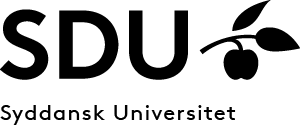
\includegraphics[width=\linewidth]{Images/scree_plot.png}
\caption{Scree plot of PCA eigenvalues, with the eigenvalue = 1 (Kaiser) cutoff.}
\label{fig:scree}
\end{figure}

Table~\ref{tab:loadings} gives the component loadings. PC1 loads positively on monocyte, lymphocyte, thrombocyte and erythrocyte and negatively on urea and coagulation factor -- a general cellular/hematologic axis. PC2 loads most strongly and positively on albumin and creatinine -- a renal/nutritional axis. PC3 loads most strongly and positively on PSA and negatively on urea -- a PSA-dominated axis distinct from the other two.

\begin{table}[H]
\centering
\caption{PCA component loadings (top-magnitude markers per PC).}
\label{tab:loadings}
\begin{tabular}{lrrr}
\toprule
Marker & PC1 & PC2 & PC3 \\
\midrule
monocyte     & 0.381  & 0.112  & $-$0.137 \\
urea         & $-$0.290 & $-$0.041 & $-$0.479 \\
lymphocyte   & 0.348  & 0.167  & 0.051 \\
thrombocyte  & 0.412  & 0.245  & $-$0.225 \\
erythrocyte  & 0.412  & 0.199  & $-$0.260 \\
albumin      & $-$0.132 & 0.593  & 0.248 \\
creatinine   & $-$0.323 & 0.532  & $-$0.047 \\
globulin     & $-$0.128 & 0.436  & $-$0.345 \\
psa          & $-$0.085 & 0.173  & 0.600 \\
coag\_factor  & $-$0.405 & $-$0.063 & $-$0.296 \\
\bottomrule
\end{tabular}
\end{table}

Keeping 3 of 10 markers as components (a $70\%$ dimensionality reduction) retains roughly two-thirds of the panel's variance, which is a reasonable trade-off for use as predictors in a downstream model, at the cost of losing direct clinical interpretability of any single original marker.

% CONCLUSION
\section{Conclusion}

\textbf{Interpretation.} A single, merged, imputed cohort table was produced from three heterogeneous sources without patient loss. PSA alone is a moderate (AUC = 0.670), not strong, discriminator of metastasis; no single cutoff is simultaneously sensitive and specific, and the "right" cutoff depends on the clinical use case (screening favours the low, high-sensitivity cutoff; confirmation favours the high, high-specificity cutoff). The ten-marker biochemical panel compresses to three interpretable components (cellular/hematologic, renal/nutritional, PSA-dominated) retaining 69.3\% of variance.

\textbf{Outcome.} Module 1.1 delivered a clean, merged, analysis-ready dataset (\texttt{DATASET123}). Module 1.2 delivered a quantified PSA performance profile and a reduced 3-component representation of the biomarker panel (\texttt{DATASET\_with\_PCA.csv}).

\textbf{Impact.} These outputs directly enable the next modelling step: the PCA components (or the raw imputed markers) and the demographic/comorbidity variables together form the feature set for a metastasis classifier, and the ROC/Youden analysis gives a defensible, data-driven cutoff instead of an arbitrary one.

\textbf{Limitations and future steps.} The mean-vs-median imputation discrepancy identified in Section~3.5 should be corrected (re-run with true median imputation and confirm downstream results are stable to the choice). PSA alone is an insufficient classifier (AUC 0.670); Module 1.3 -- feature selection over the full merged/PCA-reduced dataset and a multivariable classification model, evaluated via a confusion matrix -- was not carried out in this work and is the natural next step to improve on single-marker performance.

\end{multicols*}
\section{annexe}
\begin{figure}[H]
\centering
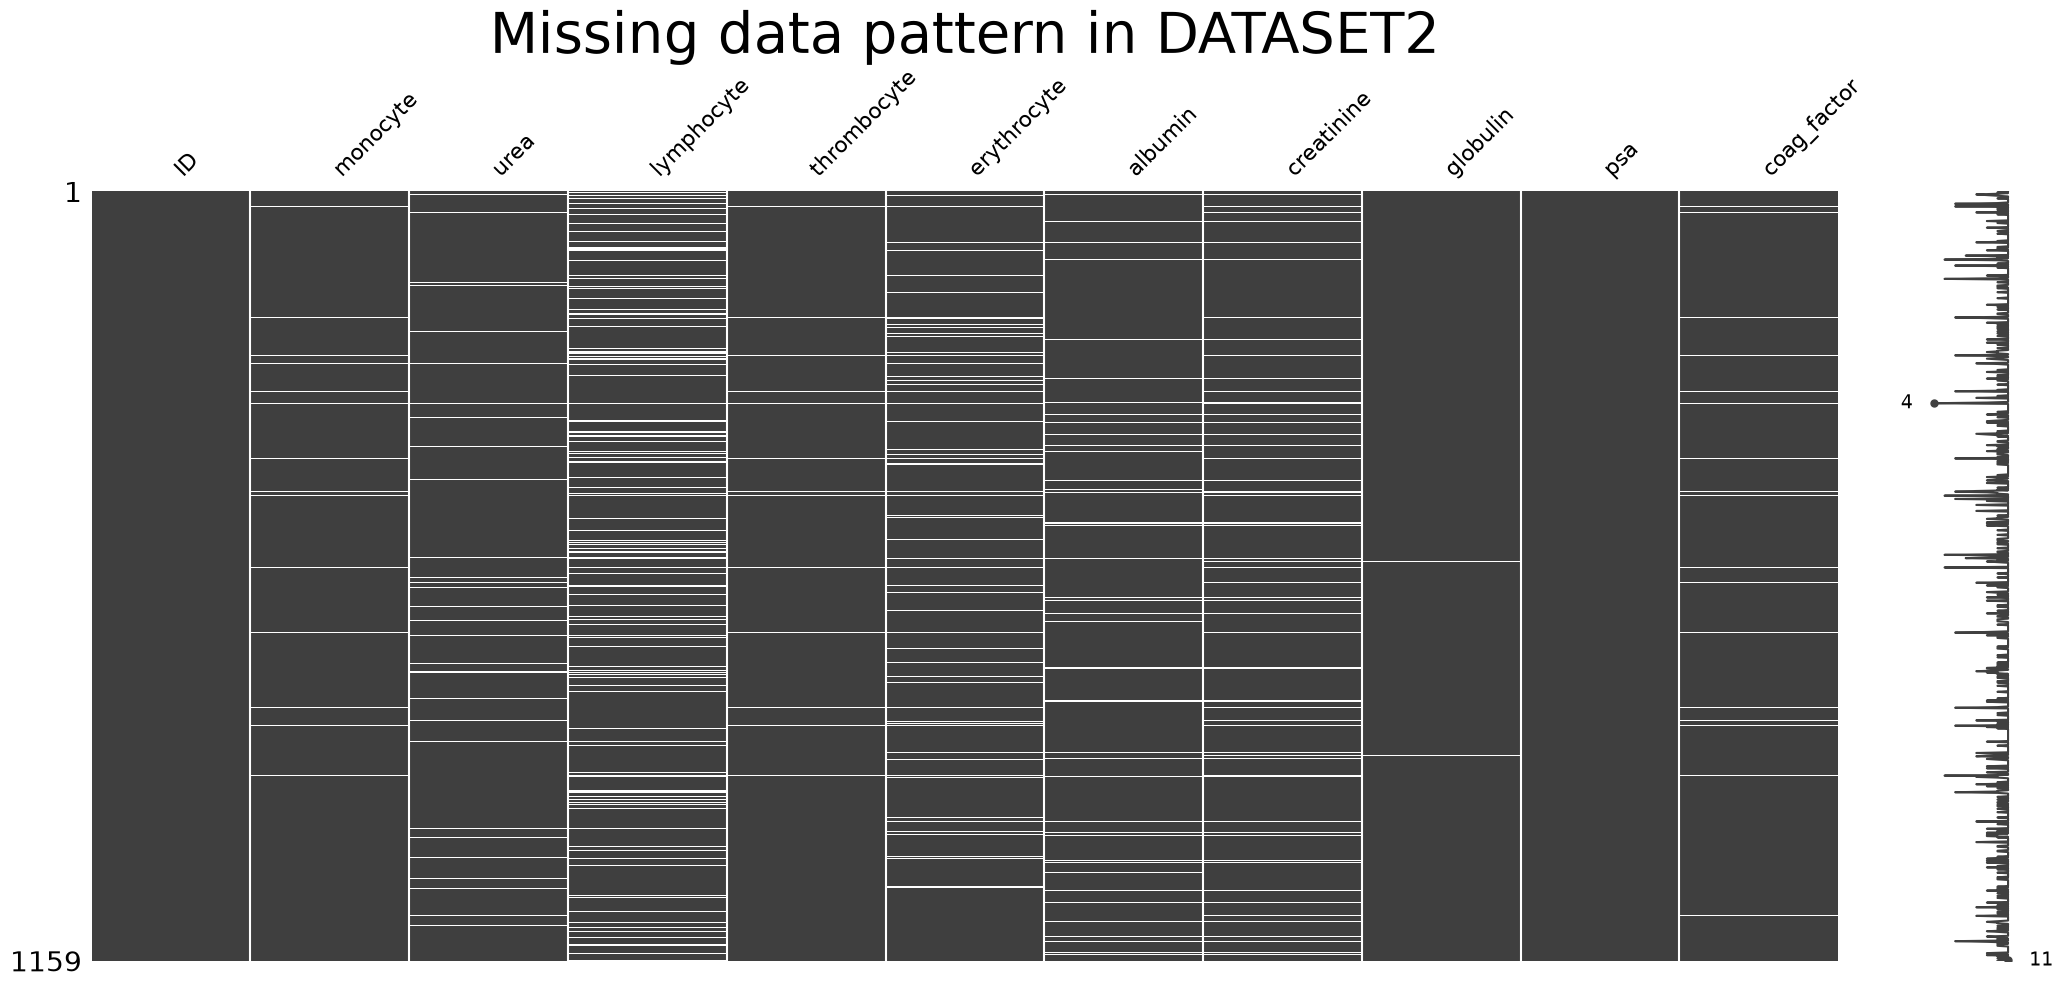
\includegraphics[width=\linewidth]{Images/missing_matrix.png}
\caption{Missingness pattern across DATASET2. Gaps are scattered rather than block-structured, consistent with values missing at random rather than missing systematically for a patient subgroup.}
\label{fig:missmat}
\end{figure}
\end{document}